\section{Emerging-market firms at equal quality}\label{sec:survival}

\paragraph{Main estimates.} Table~\ref{tab:survival} reports the extra domestic gap in emerging-market offices,
measured as survival to eight years after grant. Without quality controls it is $-10.1$ (1.5) points: domestic
firms' patents in emerging-market offices are much less cited than foreign ones. With citation slopes, field and
owner-group effects it becomes $+4.3$ (1.5). The estimate is the same for the original set of offices
(China, Korea and the four largest advanced economies) and close to zero, $-0.5$ (1.9), when Korea and Taiwan, the
two high-income members of the emerging-market group, are left out. Richer quality controls (blocking citations, citations
by age four and office-specific slopes in the grant lag) lower the estimates for every firm size by 2--3 points
(Appendix Table~
ef{tab:rich}). Small emerging-market firms then come out 1.6 (0.6) points behind, and 3.0 (0.7)
with family size, which itself partly reflects owners' capacity to file abroad; larger firms remain 4--9 points
ahead. Small firms thus keep their patents about as long as small firms in the advanced economies, within a few
points either way, and larger firms longer.

\begin{table}[t]
\centering
\begin{threeparttable}
\caption{Extra domestic--foreign survival gap in emerging-market offices (percentage points)}\label{tab:survival}
\small
% Source: em-patent-value output/ext_overall.csv, ext_gradient.csv (23_extended_offices.py)
\begin{tabular}{lccc}
\toprule
 & All ten offices & Original six & Without Korea, Taiwan \\
 & (1) & (2) & (3) \\
\midrule
\multicolumn{4}{l}{\emph{A. All firms and universities}} \\
Alive 10 years from filing, raw            & $-18.4$ (1.6) & $-19.9$ (1.8) & $-25.8$ (2.1) \\
Alive 10 years from filing, quality controls & $-5.1$ (1.4) & $-6.2$ (1.5) & $-9.0$ (1.9) \\
Alive 8 years from grant, raw              & $-10.1$ (1.5) & $-11.5$ (1.7) & $-18.5$ (2.0) \\
Alive 8 years from grant, quality controls & \textbf{4.3} (1.5) & \textbf{4.3} (1.5) & $-0.5$ (1.9) \\
\addlinespace
\multicolumn{4}{l}{\emph{B. By owner group, alive 8 years from grant, quality controls}} \\
Firms, 1--9 families     & 1.7 (0.5)    & 3.4 (0.6)    & 2.6 (0.6) \\
Firms, 10--99            & 8.2 (0.9)    & 9.8 (1.0)    & 7.8 (1.2) \\
Firms, 100--999          & 9.3 (1.7)    & 12.3 (2.0)   & 10.1 (2.8) \\
Firms, 1{,}000+          & 9.3 (3.4)    & 6.6 (3.5)    & 4.8 (6.4) \\
Universities             & $-5.7$ (3.6) & $-11.5$ (3.1) & $-16.3$ (3.0) \\
\addlinespace
Patents                  & 2{,}961{,}829 & 2{,}615{,}050 & 2{,}439{,}754 \\
\bottomrule
\end{tabular}
\begin{tablenotes}\footnotesize
\item \emph{Notes:} Coefficient $\delta$ of equation~\eqref{eq:did}; standard errors clustered by owner in
parentheses. Raw: office $\times$ filing-year effects only. Quality controls: office-specific citation slopes, office
$\times$ field and (panel A) office $\times$ owner-group effects. Column (1): China, Korea, Russia, Taiwan and the Czech
Republic against the United States, Japan, Germany, the United Kingdom and France. Column (2): China and Korea against
the United States, Japan, Germany and the United Kingdom. Column (3): column (1) without Korea and Taiwan.
\end{tablenotes}
\end{threeparttable}
\end{table}

\paragraph{By country.} Figure~\ref{fig:country} compares each emerging-market office with the five advanced-economy
offices, by owner group. Chinese and Korean firms of every size are ahead: small firms by 4.0 (0.6) and 1.7 (1.1)
points, larger firms by 8--12 points. Czech firms are ahead by similar amounts, though with wide intervals. Russia is
the exception: small Russian firms are 5.9 (1.5) points behind, and Russian universities 11.9 (4.7). Small Taiwanese
firms are 3.8 (1.5) points behind, while large Taiwanese firms and universities are well ahead. Even the Russian and
Taiwanese shortfalls sit inside the range of domestic--foreign gaps among small firms in the advanced-economy
offices, from about zero in the United Kingdom to 18 points in Japan (Appendix Table~\ref{tab:within}).

\begin{figure}[t]
\centering
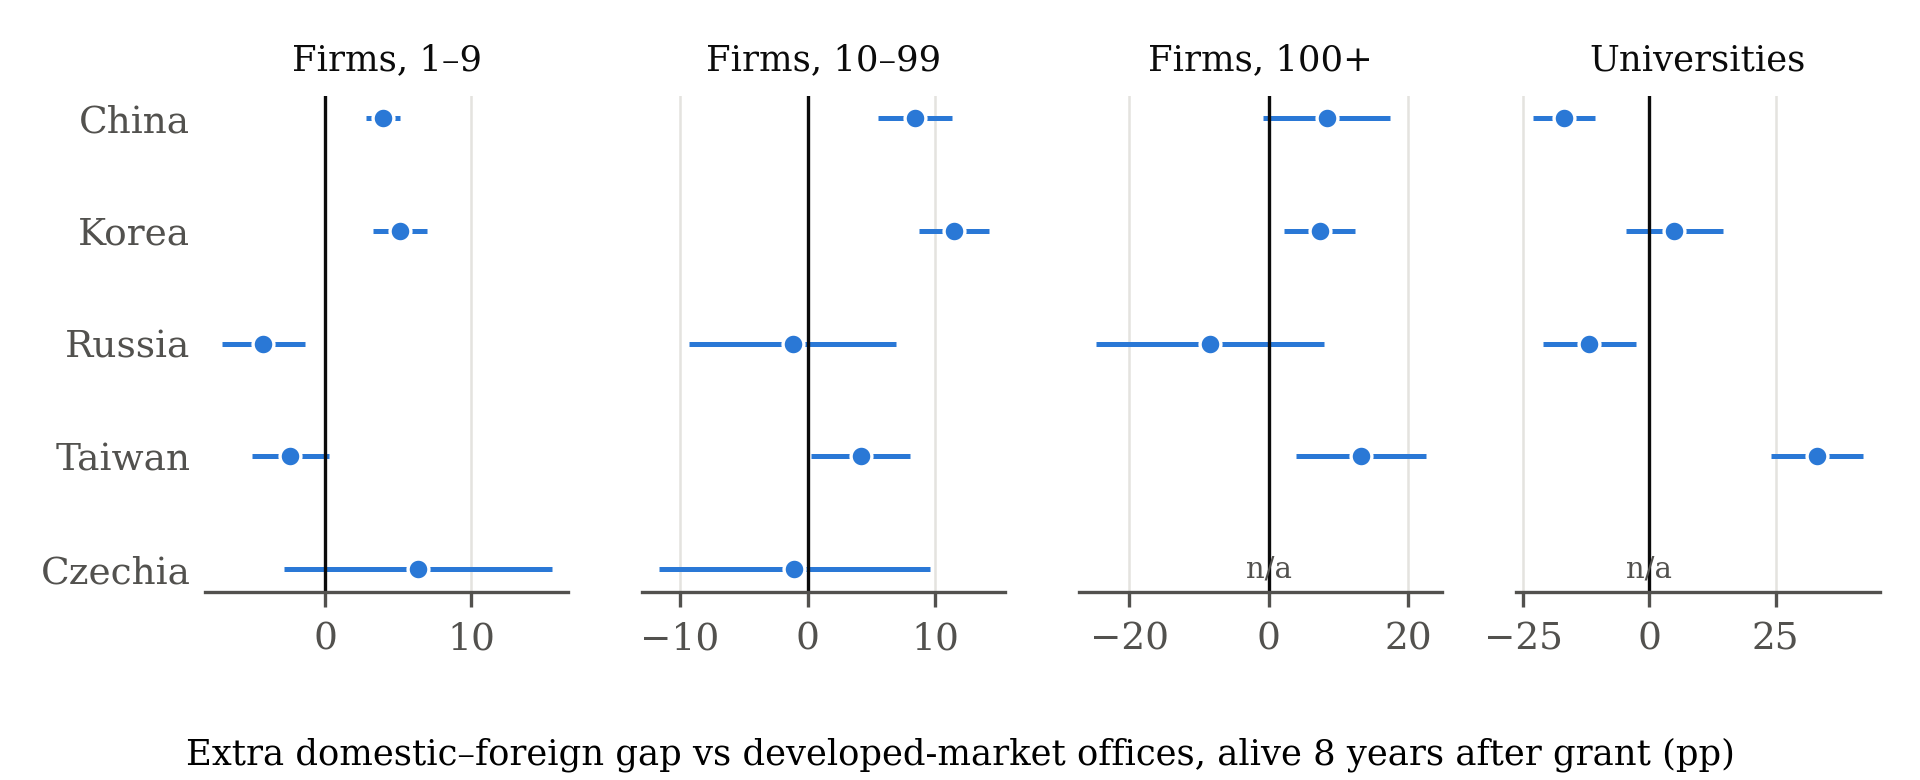
\includegraphics[width=0.9\textwidth]{figures/fig3_by_country.png}
\caption{Each emerging-market office against the advanced-economy offices}\label{fig:country}
\figurenotes{Coefficient $\delta$ of equation~\eqref{eq:did} estimated on one emerging-market office and the five
advanced-economy offices, separately for each owner group, with 95\% confidence intervals (standard errors clustered
by owner). Outcome: alive eight years after grant. The Czech Republic has too few domestic university patents (95).}
\end{figure}

\paragraph{Same invention, home and abroad.} Inventions patented both at home and in another study office hold the
technology fixed. With patent-family fixed effects, I compare how much longer small firms keep the home patent than
the same invention's foreign patents, relative to larger firms from the same country. If small emerging-market firms
found their home patents hard to use, they would drop them first. They do the opposite: small firms keep the home
patent relatively longer in China, by 10.2 (3.8) points, and Korea, by 9.9 (2.0), as in Japan (14.9), France (6.6)
and the United States (4.4); in Taiwan the difference is close to zero and in Russia it is imprecise (Appendix
Table~
ef{tab:same}). Small owners everywhere economise on
the expensive foreign patent first.

\paragraph{Credit shocks.} If finance were binding, credit crunches should raise small domestic firms' lapses. In a
patent-year panel with country-specific shock years (banking crises and documented credit crunches;
\citealp{LaevenValencia2018}), the interaction of shock, small owner and domestic owner is 0.37 points per year (0.75)
in the emerging-market offices and 0.23 (0.52) in the advanced-economy ones (Appendix Table~
ef{tab:credit}). Office $\times$ year effects
absorb fee changes and recording practices.

\paragraph{Fees.} Fee changes test cash constraints at renewal time directly. China's 85\% fee reduction for small
owners, whose window was extended from three to six fee-years in 2016 and to ten in 2018, lowers small firms' lapse
rate only slightly: an implied elasticity of 0.07 (intent to treat, since take-up is not observed). Small US firms
respond to stage-specific maintenance-fee changes with an elasticity of about 0.18. Small emerging-market firms are
not more fee-sensitive than small US firms.

\paragraph{Sales.} One result points to owner capacity at the margin. In a landmark design (patents alive and not
yet sold at ages 4--8, sold in the next year or not, outcome alive five years later, with citations counted only up
to the landmark age), a sale raises survival by 4.7 (0.7) points on average, by a further 8.3 (1.0) for small
emerging-market firms and by only 0.8 (1.0) for small advanced-economy firms
(Appendix Table~\ref{tab:credit}, panel B). Buyers select good patents everywhere, so the level of the premium is not causal;
the extra premium for small emerging-market sellers is the informative part. In China it is largest for sales to
other firms; in Russia there is none. Taiwan and the Czech Republic record no ownership transfers.
